
\chapter{Stand der Technik}
\section{Andere Lösungen}
Das Ziel des praktischen Teils der Bachelorarbeit ist es, die Informationen der Statischen Code Analyse übersichtlicher, dauerhafter und benutzerfreundlicher zu präsentieren. Hierbei gibt es ähnliche bereits bestehende Lösungen, deren Probleme im Punkt 2.3.2 Probleme aufgezeigt werden: 

\subsection{Entwicklungsumgebungen}
Bestehende Entwicklungsumgebungen zeigen die Informationen und Warnung bezüglich Fehler und Regelverletzungen zur Übersetzungszeit auf. Dies geschieht in der Zeile bzw. bei der Fehlerquelle, in der sich der Fehler befindet. Die Informationen werden hierbei in einem kleinen Textfeld angezeigt oder gesammelt in einem Ausgabefenster angezeigt. Weitere Funktionen  sind in einigen Entwicklungsumgebungen extra ergänzt, zum Beispiel die Funktion des automatischen Navigierens von der Übersichtsliste in die Fehlerzeile. Beim Durchführen der Statischen Code Analyse in Entwicklungsumgebungen spricht man von einem \textit{On-Demand-Scan}, da der Entwickler oder die Entwicklerin das Tool für die Analyse manuell startet. Um die Statische Code Analyse in einer Entwicklungsumgebung verwenden zu können, müssen spezifische Tools installiert werden. So bieten Entwicklungsumgebung wie IntelliJ IDEA oder Visual Studio die Möglichkeit Plugins wie SonarLint oder Checkstyle zu installieren. \cite{sonarLint}
\begin{figure}[tp]
  \centering
  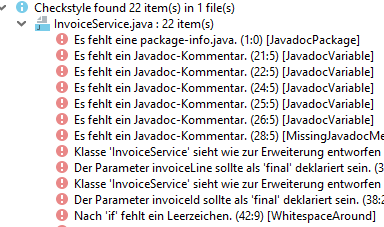
\includegraphics[height=7cm]{images/ideChecks.PNG}
  % The short caption should be capitalised
  % The full caption should hold a full sentence. 
 \caption[Anzeige von Fehler in der Entwicklungsumgebung Intellij IDEA]{Anzeige von Fehler in der Entwicklungsumgebung Intellij IDEA.}
  \label{fig:engine}
\end{figure}
\subsection{Build-Server und Continuous Integration (CI)-Pipeline}
Die Statische Code Analyse wird auch bei Build-Server in der CI-Pipeline verwendet. \cite{zampetti2017open} Der Vorteil dabei ist, dass der Entwickler die Tools nicht lokal installieren muss. Die Tools oder die Plugins werden direkt am Build-Server installiert. Die Code Analyse wird direkt beim automatischen Build durchgeführt. Um diese Option verwenden zu können, gibt es auf Build-Server verfügbare Plugins, wie zum Beispiel das Plugin \textit{Fortify}, dass auf der Build-Server Lösung Jenkins installiert werden kann.
\subsection{SonarQube}
Die Software SonarQube prüft und analysiert das Programm auf bestimmte Faktoren und Regeln. SonarQube fokussiert sich hierbei nicht nur auf die Statische Code Analyse, sondern auch auf dynamische Tests. Die Ergebnisse der Prüfungen und Analyse werden hierbei auf einer Website angezeigt. SonarQube kann sowohl lokal am Rechner, sowie auf einem Build-Server installiert und verwendet werden. Bei einer Installation am Build-Server werden im Zuge des Build-Prozesses auch die SonarQube Prüfungen und Tests durchgeführt. SonarQube unterstützt eine Vielzahl an Programmiersprachen wie Java, C oder C++. Je Projekt können auf der Website die Fehler, Test-Coverage, Duplications und eine weitere Faktoren eingesehen werden. Die Meldungen werden zusätzlich in verschiedene Gewichtige eingeteilt: Blocker, Critical, Info und Minor. \cite{sonarQubeHeise}

\begin{figure}[tp]
  \centering
  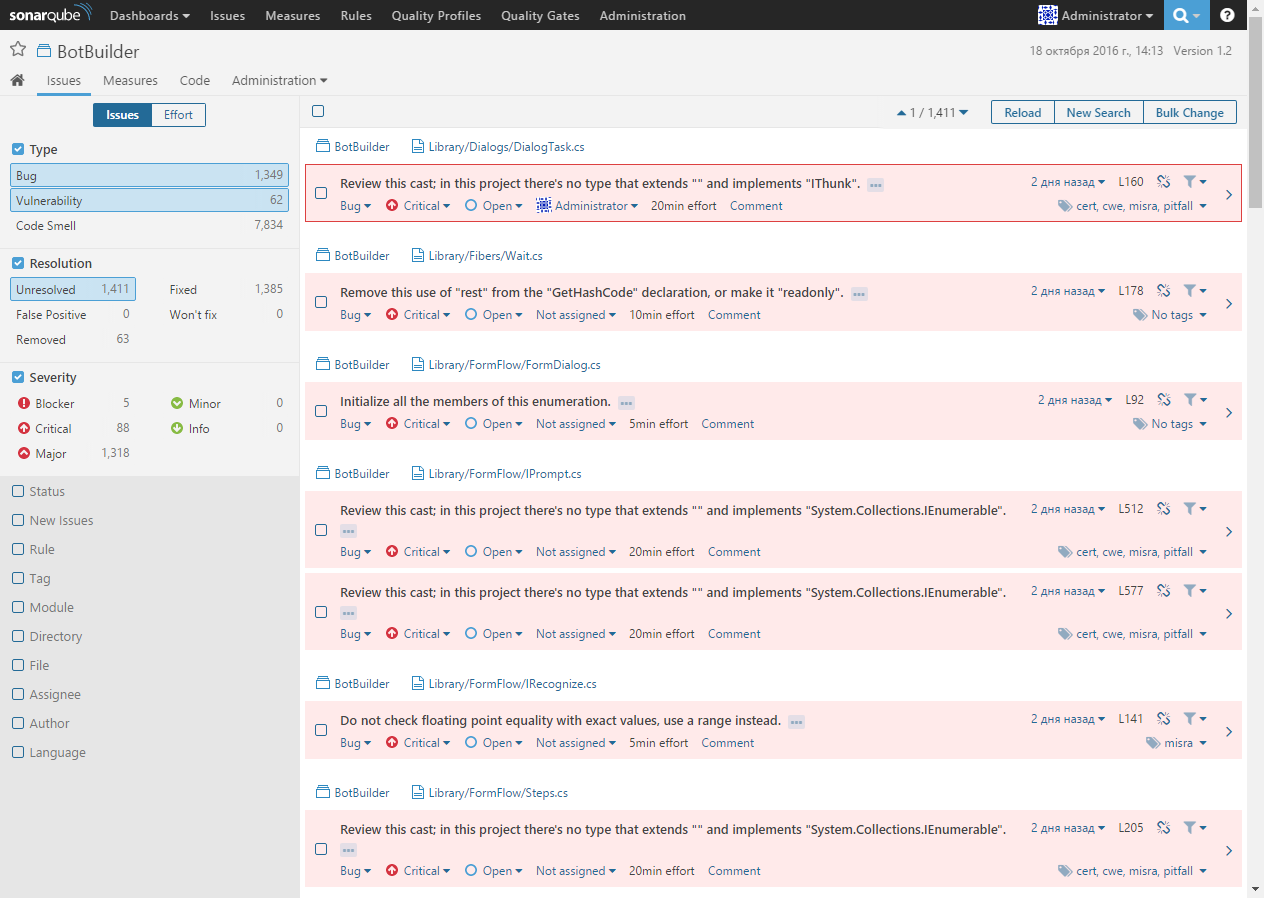
\includegraphics[height=8cm]{images/sonarQube.PNG}
  % The short caption should be capitalised
  % The full caption should hold a full sentence. 
 \caption[Anzeige von Fehlern und Problemen eines Projekts im SonarQube]{Anzeige von Fehlern und Problemen eines Projekts im SonarQube.}
  \label{fig:engine}
\end{figure}

\subsection{Veracode}
Vercode ist eine Software-Lösung, die den Code auf Security-Lags und anderen Problemen untersucht. Auch wird eine \textit{Software Composition Analysis} durchgeführt. Hierbei werden eingesetzte Open Source Tools auf Sicherheitslücken untersucht. Um eine Veracode-Analyse durchführen zu können, wird der Code auf eine bereitgestellte Website hochgeladen und dort automatisch analysiert und untersucht. Die Ergebnisse sind auf der Website einsehbar. Veracode arbeitet wie SonarQube mit dynamischen und statischen Tests, kann aber auch in Entwicklungsumgebungen eingebunden werden. Ebenso werden eine Vielzahl an Programmiersprachen unterstützt.  \cite{veracodeDig}  

\section{Statische Code Analyse}
Die Code Analyse ist die Analysemöglichkeit des Quellcodes auf Fehler. Dazu ist Statische Code Analyse ist die Analysemöglichkeit des Quellcodes zur Übersetzungszeit. In dieser Analyse werden Prüfungen durchgeführt, die bestimmte Fehler, Regeln und Attribute identifizieren und aufzeigen. \cite{gomes2009overview}
Die Statische Code Analyse soll ein gute Code-Qualität sicherstellen. Für die Beschreibung einer guten Code-Quality gibt es mehrere Modelle, wie das McCall Model, Boehm Model pder das ISO/IEC Proposed Model. Diese Modelle definieren bestimmte Faktoren, die für eine gute Code-Qualität wichtig sind: Portabilität, Wiederverwendbarkeit, Interoperabilität, Korrektheit, Zuverlässigkeit, Effizienz, Integrität, Benutzerfreundlichkeit, Testbarkeit, Flexibilität und Wartbarkeit. Diese Faktoren werden von allen Modellen als bestimment hervorgehoben, die Modelle unterscheiden sich aber untereinander, wie zum Beispiel bei den Faktoren Dokumentation und Resilience. \cite{iqbalCodeQualityApproach}
Eine gute Code-Qualität kann aber nie durch Tools alleine sichergestellt werden, sondern es erfordert auch manuelle das Testen der Software. 
\subsection{Unterschiede zu dynamischen Tests}
Im Gegensatz zur Statische Code Analyse überprüft die dynamische Code Analyse dynamischen und variablen Aspekte des Programms. Mit verschiedenen Eingabeparametern wird auf ein bestimmtes Ergebnis getestet. \cite{grigorenkoDynTest} Für diese Tests wird eine Simulation erstellt bzw. gestartet. Aus diesem Grund benötigt ein dynamischer Test ein lauffähiges Programm, was bei einem statischen Test nicht vorausgesetzt wird. Ein dynamischer Test auf zwei verschiedene Arten durchgeführt werden: Als Black-Box, White-Box oder diversifizierender Test.
In der Methode des Black-Box-Testings ist das zu testende System der Testerin oder dem Tester nicht bekannt. Hierbei wird ausschließlich die Funktionalität anhand der Spezifikationen getestet. Bei White-Box-Tests ist das System und der Code bekannt, daher sind die ausführenden Tester oft Entwicklerinnen und Entwickler des Programms. Anhand des Programms werden daher Tests erstellt, die bestimmte Teile überprüfen und testen sollen. Bei diversifizierenden Tests hingegen, werden die Testergebnisse nicht mit der Spezifikation verglichen, sondern sie vergleichen verschiedene Versionen der Software. Sind die getesteten Version gleich, so ist der Testfall erfolgreich. Ein diversifizierenden Test kann entweder als Back-to-back-Test (Testen von verschiedene Lösungen und Versionen des Programms), Regressionstest (Wiederholen des selben Tests um sicherzustellen, dass bereits getestete Software-Teile keine neuen Fehler aufweisen) oder als Mutationtest (Leistungsfähigkeit der Testmethoden) durchgeführt werden. \cite{bommer2016softwarewartung}\\
Um eine hohe Qualität des Programms zu gewährleisten, müssen daher beide Testverfahren kontinuierlich betrieben werden.
\section{Tools für die Statische Code Analyse}
Für die Statische Code Analyse gibt es eine Vielzahl an Anwendungen und Programmen. Diese Tools können Programmiersprachen-abhängig sein, es gibt aber auch Sprachen übergreifende Lösungen. Die Tools können für allgemeine Code-Smells, aber auch Lösungen für bestimmte Einsatzgebiete sein. Die Entwickler und Entwicklerinnen müssen für  spezifische Probleme und Faktoren bestimmte Tools einsetzten:

\begin{itemize}
\item \textbf{Code-Qualität} beschreibt, ob das Programm seine Funktionen richtig und effizient ausführt. Aber auch Leerzeichen und die Länge von Methoden und Klassen fallen in diese Kategorie. Tools für diese Einsatzbereiche sind CheckStyle oder FindBugs. Aber auch der Faktor der Wiederverwendbarkeit (Hinzufügen von neuen Features, Verwendbarkeit des Codes für andere Entwicklerinnen und Entwickler) fällt in diese Kategorie. Die Tools Jalopy und Jar analyser testen den Code auf die Möglichkeit der Wiederverwendbarkeit. 
\item \textbf{Nebenläufigkeit}
beschreibt die Möglichkeit, mehrere Funktionen zur selben Zeit auszuführen. Tools wie Sonar oder CheckThread untersuchen den Code hierbei auf Probleme, wie zum Beispiel ein falsches Thread-Handling. 
\item \textbf{Abhängigkeiten}
Beschreibt die Abhängigkeit eines Software-Moduls zu einem anderen Modul. In einer Programm solten wenige abhängigkeiten auftreten, da diese bei Ausfall Fehler oder Verzögerungen hervorrufen. Um Abhängigkeitsfehler wie Zirkulationen vorzubeugen, können Tools wie JDepend oder Dependecy Finder eingesetzt werden.
\item \textbf{Exception-Handlingg} Mit dem Exception-Handling können Software-Fehler gefangen werden. Um werden Fehler aber nicht geworfen und die Exception-Blocks sind redundant aufgebaut. hier können Tools wie JLint eingesetzt werden
\item \textbf{Kompatibilität} Richtige Kompatibilität zwischen Source- und Binary Code kann mit Tools wie Clirr sichergestellt werden. 
\item \textbf{Code-Style} Mit Style werden bestimmte Regeln und Coding-Conventions verstanden. Unter anderem gehören dazu Bestimmungen zu Leerzeichen, Klammern und Namenskonventionen. Für die Überprüfung des Code-Styles können Tools wie CheckStyle oder PMD eingesetzt werden.
\item \textbf{Speicherlecks}
Bei einem Speicherleck (memory leak) sind Daten im Arbeitsspeicher gespeichert,  welche aber nicht verwendet oder gelöscht werden. Tools wie Coverity können das Entstehen von Speicherlecks verhindern.
\item \textbf{Race Conditions}
Bei einer Race Condition greifen zwei verschiedene Services auf eine Ressource oder Methode zu. Deswegen kann nur eine der beiden Services das Ziel verwenden. Das andere Service kann die Ressource nicht verwenden, was zu einem Fehler oder einem unerwünschten Ergebnis führen kann. Dieses Problem kann bei Threads auftreten. Tools wie JLint oder ConTest können ein Race Condition-Problem feststellen.
\item \textbf{Security}
Security ist ein wichtiger Punkt in Programmen. Tools wie FindBugs, Protecode und Xanitizer analysieren den Code und können Sicherheitsprobleme aufdecken, beispielsweise hard coded Passwörter, (Command) Injection und Response Splitting. \cite{goseva2015capability} Eine hierbei verwendete Technik ist die Taint-Analyse, wo der Datenfluss einer Dateneingaben überprüft wird. \cite{jung2014sensitive}
\end{itemize}

Um die einzelnen Tools bewerten und vergleichen zu können, müssen sie daher in verschiedene Anwendungsbereiche geteilt werden. Bei einer Bewertung der Tools sind aber auch andere Metriken ausschlaggebend wie: Möglichkeit der Erweiterbarkeit der Tools (Open-Source), letztes Release und Art und Vielfalt der Reports.\cite{comparativeAnalysisTools}

\section{Anzeige der Analyse} 
xml report, ide anzeige, 
\subsection{Probleme} 

\subsubsection{Keine dauerhafte Anzeige} 
Der Fokus der Anzeige der Analyse der Statischen Code Analyse in Entwicklungsumgebungen liegt auf die Fehlerausbesserung. Die Fehler und Informationen werden daher nach der Ausbesserung nicht mehr angezeigt. Die Entwicklerin oder der Entwickler kann die ausgebesserten Fehler nicht mehr einsehen.

\subsubsection{Keine Verbesserung des Entwicklers} 
Da die Fehler nicht dauerhaft angezeigt werden, kommt es zu keiner Verbesserung der Programmierkenntnisse der Entwickler und Entwicklerinnen. Weiters kann in Entwicklungsumgebungen die automatische Ausbesserung getätigt werden, sodass der Entwickler oder die Entwicklerin oft den Fehler nicht bewusst überdenken und selber ausbessern wird. 
Die selben Fehler häufen sich daher immer wieder. Dies geschieht auch, weil besonders unerfahrenere Entwickler einige Fehlerwarnung nicht nachvollziehen und verstehen können, da es keine Möglichkeit gibt die Bugs genauer einsehen zu können. 

\subsubsection{Unübersichtliche Anzeige} 
In großen Klassen, wo sich viele Fehler und Informationen befinden, gehen die einzelnen Fehler in der kleinen Übersichtsanzeige oft unter. In der Zeile, wo sich der Fehler befindet, kann der Fehler nur mit einem Hover über die Warnung angezeigt werden. 